\documentclass[11pt]{article}
\usepackage[margin=1in]{geometry}
\usepackage{booktabs}
\usepackage{graphicx}
\usepackage{subcaption}
\usepackage{float}
\usepackage{longtable}
\usepackage{array}
\usepackage{hyperref}
\usepackage{enumitem}

\title{KinBench-UQ: Realistic Kinase--Ligand Candidate Prioritization with Exact Literature Baselines and Reproducible Evidence}
\author{}
\date{}

\begin{document}
\maketitle

\begin{abstract}
Drug--target affinity work for kinases is often evaluated on optimistic
interaction-level splits and summarized with aggregate error metrics that do
not directly answer the candidate-prioritization question faced by
experimentalists. We present KinBench-UQ, a reproducible benchmark for
kinase--ligand prioritization that combines exact sequence-identity-aware
splitting, mutation-family analysis, external validation, literature-style
reproductions, and generated paper artifacts. The current benchmark compares
five models under a shared protocol: \texttt{ligand\_only\_ridge},
\texttt{ridge\_ensemble}, \texttt{dual\_tower\_uq}, \texttt{deepdta\_exact},
and \texttt{graphdta\_gcn\_exact}. The results show a nontrivial trade-off
landscape rather than a trivial single-model win: \texttt{deepdta\_exact} is
strongest on the easier random split and attains the best RMSE on the exact
sequence-identity split, whereas \texttt{dual\_tower\_uq} is strongest on the
harder cold-target and mutation-holdout settings and retains the best Spearman
correlation on several realistic splits. All primary tables and figures are
generated from saved result artifacts under \texttt{results/} rather than
typed manually into the manuscript.
\end{abstract}

\section{Introduction}

Kinase inhibitor discovery is not only a regression problem. In practice, a
scientist wants to know which compounds should be tested first for a target of
interest, often under budget constraints and often for targets or variants that
are not cleanly represented by the training distribution. Standard DTA
benchmarks such as Davis and KIBA have been useful for model development, but
they also encourage a narrow evaluation habit: optimize a global error metric
under a split that may retain substantial target similarity between training
and test sets.

KinBench-UQ is built around a stricter and more scientist-facing question:

\begin{quote}
Under realistic train--test separation, which model best prioritizes kinase
compounds, and how reproducible is the resulting evidence?
\end{quote}

The repository aims to contribute on two axes at once. First, it provides a
target-aware benchmark with realistic split families, leakage analysis,
mutation-family analysis, and external validation. Second, it packages that
benchmark in a reproducible way: the result summaries, figures, and manuscript
fragment are generated directly from versioned result files.

\section{Task and Data}

\subsection{Task Definition}

Given a ligand and a kinase target, the system predicts binding strength in the
form of \texttt{p\_activity}. These predictions are used for regression-style
evaluation and, more importantly, for ranking candidate compounds for a target.
The problem is therefore best understood as a target-aware candidate
prioritization task, not merely a curve-fitting exercise.

\subsection{In-Domain Dataset}

The primary benchmark dataset is Davis, containing 30,056 ligand--target
affinity measurements over 68 ligands and 442 kinase targets. The raw affinity
values are standardized into
\[
\texttt{p\_activity} = -\log_{10}(\text{affinity in molar units}),
\]
while the original assay family is preserved explicitly in
\texttt{affinity\_type}. This is important because the benchmark is designed to
support future mixed-assay extensions without silently mislabeling the target
variable.

\subsection{External Validation Dataset}

The external test set is built from BindingDB-derived kinase measurements,
processed into the same schema as Davis. The current external panel contains
1,617 rows, 8 targets, and 1,296 unique ligands after cleaning and
deduplication. The current external build retains \texttt{KD} measurements for
closer comparability to Davis.

\section{Benchmark Design}

\subsection{Why More Than One Split Is Needed}

A single easy split can produce misleadingly optimistic conclusions. A model
may appear to generalize while still benefiting from near-duplicate target
context, dataset-specific regularities, or evaluation scenarios that do not
match the intended use case. To address this, KinBench-UQ evaluates multiple
split families that test different types of generalization.

\subsection{Primary Split Families}

The current paper focuses on four primary split families:

\begin{itemize}[leftmargin=1.5em]
  \item \textbf{Random}: standard interaction-level holdout.
  \item \textbf{Cold-target}: evaluation targets do not appear in training.
  \item \textbf{Sequence-identity}: targets are separated using exact global
  pairwise sequence identity and clustered before splitting.
  \item \textbf{Mutation-holdout}: mutant family members are reserved for
  evaluation while related family context remains in training.
\end{itemize}

\subsection{Exact Sequence-Identity Control}

The sequence-identity split is a central design choice. Earlier versions of the
repository used a proxy similarity score. The current benchmark replaces that
with exact global pairwise alignment identity and stores the resulting identity
table and cluster assignments under the benchmark artifacts. The generated
leakage summary shows that the mean nearest-train identity on this split falls
to 0.367, with a maximum of 0.581, whereas several easier splits still admit
exact or near-exact target neighbors.

\section{Compared Models}

Five models are compared under a common benchmark runner.

\begin{enumerate}[leftmargin=1.5em]
  \item \texttt{ligand\_only\_ridge}: a simple molecule-only baseline.
  \item \texttt{ridge\_ensemble}: a classical target-aware baseline using
  ligand and target features.
  \item \texttt{dual\_tower\_uq}: the main repository model with explicit
  ligand-side and target-side representations plus predictive uncertainty.
  \item \texttt{deepdta\_exact}: a literature-style DeepDTA reproduction run
  under the repository protocol.
  \item \texttt{graphdta\_gcn\_exact}: a literature-style GraphDTA reproduction
  run under the same protocol.
\end{enumerate}

\subsection{Repository Model}

The repository model is implemented in
\texttt{src/kinase\_ligand\_ranking/neural\_modeling.py} as
\texttt{DualTowerUncertaintyRanker}. It combines

\begin{itemize}[leftmargin=1.5em]
  \item Morgan fingerprints for ligands,
  \item sequence-derived features for kinase targets,
  \item assay/source context features,
  \item random linear projections for ligand and target embeddings, and
  \item interaction features formed from ligand--target projected products.
\end{itemize}

These features are consumed by an \texttt{ExtraTreesRegressor}. Predictive
uncertainty is derived from per-tree prediction spread and calibrated on the
validation split.

\subsection{Feature Construction}

The repository feature pipeline, implemented in
\texttt{src/kinase\_ligand\_ranking/features.py}, encodes each row using:

\begin{itemize}[leftmargin=1.5em]
  \item 1024-bit Morgan fingerprints for ligands,
  \item amino-acid composition and sequence summary statistics for targets,
  \item one-hot assay-type features,
  \item one-hot source features.
\end{itemize}

\subsection{Why Literature Baselines Matter}

The literature baselines are not included for decoration. They are needed so
the benchmark does not reduce to ``our model on our preferred split.'' Running
DeepDTA and GraphDTA under the same protocol makes the comparison more credible
than quoting incompatible numbers from older papers.

\section{Evaluation Protocol}

\subsection{Primary Metrics}

The benchmark reports:

\begin{itemize}[leftmargin=1.5em]
  \item RMSE on \texttt{p\_activity},
  \item global Spearman correlation,
  \item mean per-target Spearman,
  \item ROC-AUC at \texttt{p\_activity >= 6.0},
  \item mean top-10\% enrichment.
\end{itemize}

RMSE measures numerical error. Spearman is especially important for the
candidate-prioritization use case because it reflects ranking quality.

\subsection{Secondary Analyses}

In addition to split-level metrics, the repository exports:

\begin{itemize}[leftmargin=1.5em]
  \item nearest-train identity leakage summaries,
  \item mutation-family performance tables,
  \item external validation summaries,
  \item uncertainty-oriented metrics for uncertainty-capable models.
\end{itemize}

\subsection{Reproducibility Path}

The intended reproducibility path is:

\begin{enumerate}[leftmargin=1.5em]
  \item create the pinned Python 3.12 environment via
  \texttt{environment.yml} or \texttt{requirements-lock.txt},
  \item build Davis and benchmark splits,
  \item run the benchmark via \texttt{scripts/run\_benchmark\_suite.py},
  \item build and run external validation via
  \texttt{scripts/run\_external\_validation.py},
  \item generate figures and paper assets via
  \texttt{scripts/generate\_paper\_assets.py}.
\end{enumerate}

The shortest command path is
\texttt{python scripts/run\_submission\_pipeline.py --device cpu}, while the
step-by-step path is documented in \texttt{docs/reproduce\_paper.md}.

\section{Results}

\subsection{Main Benchmark Results}

Table~\ref{tab:main-results} summarizes the current four-split comparison. The
most important outcome is that the benchmark produces a meaningful trade-off
landscape rather than a trivial win for one model on every axis.

\begin{table}[H]
\centering
\caption{Main benchmark results on the four primary split families. Lower RMSE
is better. Higher Spearman is better.}
\label{tab:main-results}
\begin{tabular}{llcc}
\toprule
Split & Model & RMSE & Spearman \\
\midrule
Random & deepdta\_exact & 0.548 & 0.658 \\
Random & graphdta\_gcn\_exact & 0.591 & 0.610 \\
Random & dual\_tower\_uq & 0.596 & 0.634 \\
\midrule
Cold-target & dual\_tower\_uq & 0.597 & 0.587 \\
Cold-target & deepdta\_exact & 0.614 & 0.563 \\
Cold-target & graphdta\_gcn\_exact & 0.690 & 0.478 \\
\midrule
Sequence-identity & deepdta\_exact & 0.681 & 0.446 \\
Sequence-identity & dual\_tower\_uq & 0.701 & 0.461 \\
Sequence-identity & graphdta\_gcn\_exact & 0.780 & 0.385 \\
\midrule
Mutation-holdout & dual\_tower\_uq & 0.545 & 0.818 \\
Mutation-holdout & graphdta\_gcn\_exact & 0.736 & 0.749 \\
Mutation-holdout & deepdta\_exact & 0.764 & 0.739 \\
\bottomrule
\end{tabular}
\end{table}

These results support three observations. First, \texttt{deepdta\_exact} is
the strongest model on the easier random split. Second, the harder
\texttt{cold\_target} and \texttt{mutation\_holdout} settings favor
\texttt{dual\_tower\_uq}. Third, the exact sequence-identity split produces a
more nuanced picture: \texttt{deepdta\_exact} is slightly best by RMSE, while
\texttt{dual\_tower\_uq} is slightly best by Spearman.

\subsection{Split Difficulty and Leakage}

The identity leakage analysis confirms that split choice changes the meaning of
the benchmark. The \texttt{sequence\_identity} split is the only primary split
with a materially reduced nearest-train identity ceiling. This is visible in
Figure~\ref{fig:leakage} and explains why the sequence-aware setting is a more
convincing generalization test than standard random holdout alone.

\begin{figure}[H]
\centering
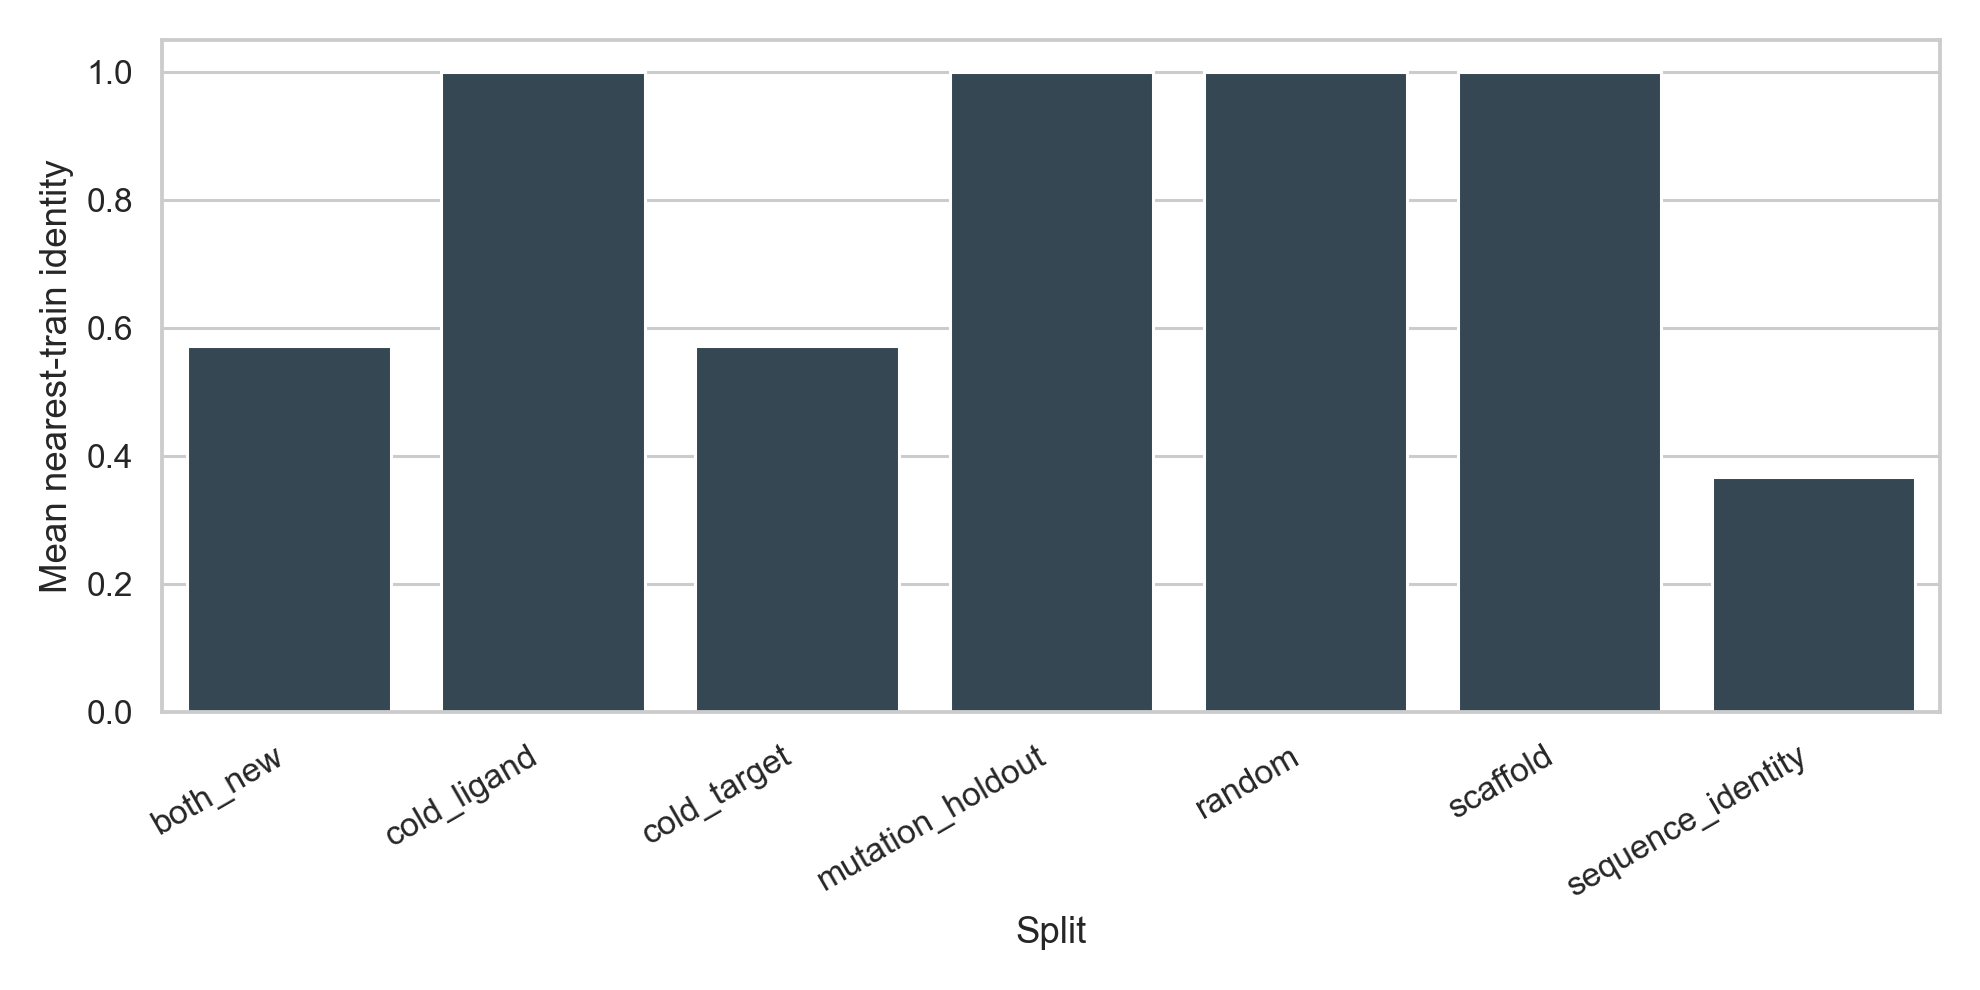
\includegraphics[width=0.8\linewidth]{../figures/sequence_identity_leakage.png}
\caption{Mean nearest-train sequence identity across split families.}
\label{fig:leakage}
\end{figure}

\subsection{Mutation-Family Analysis}

The mutation-family table shows that aggregate performance hides meaningful
family-level variation. The repository model is especially strong on several
families, including PIK3CA (RMSE 0.150), LRRK2 (0.334), BRAF (0.389), MET
(0.411), and FLT3 (0.520). In contrast, both literature baselines degrade more
substantially on multiple family groups. This is practically important because
resistance and variant-focused kinase work is often family-specific.

\begin{figure}[H]
\centering
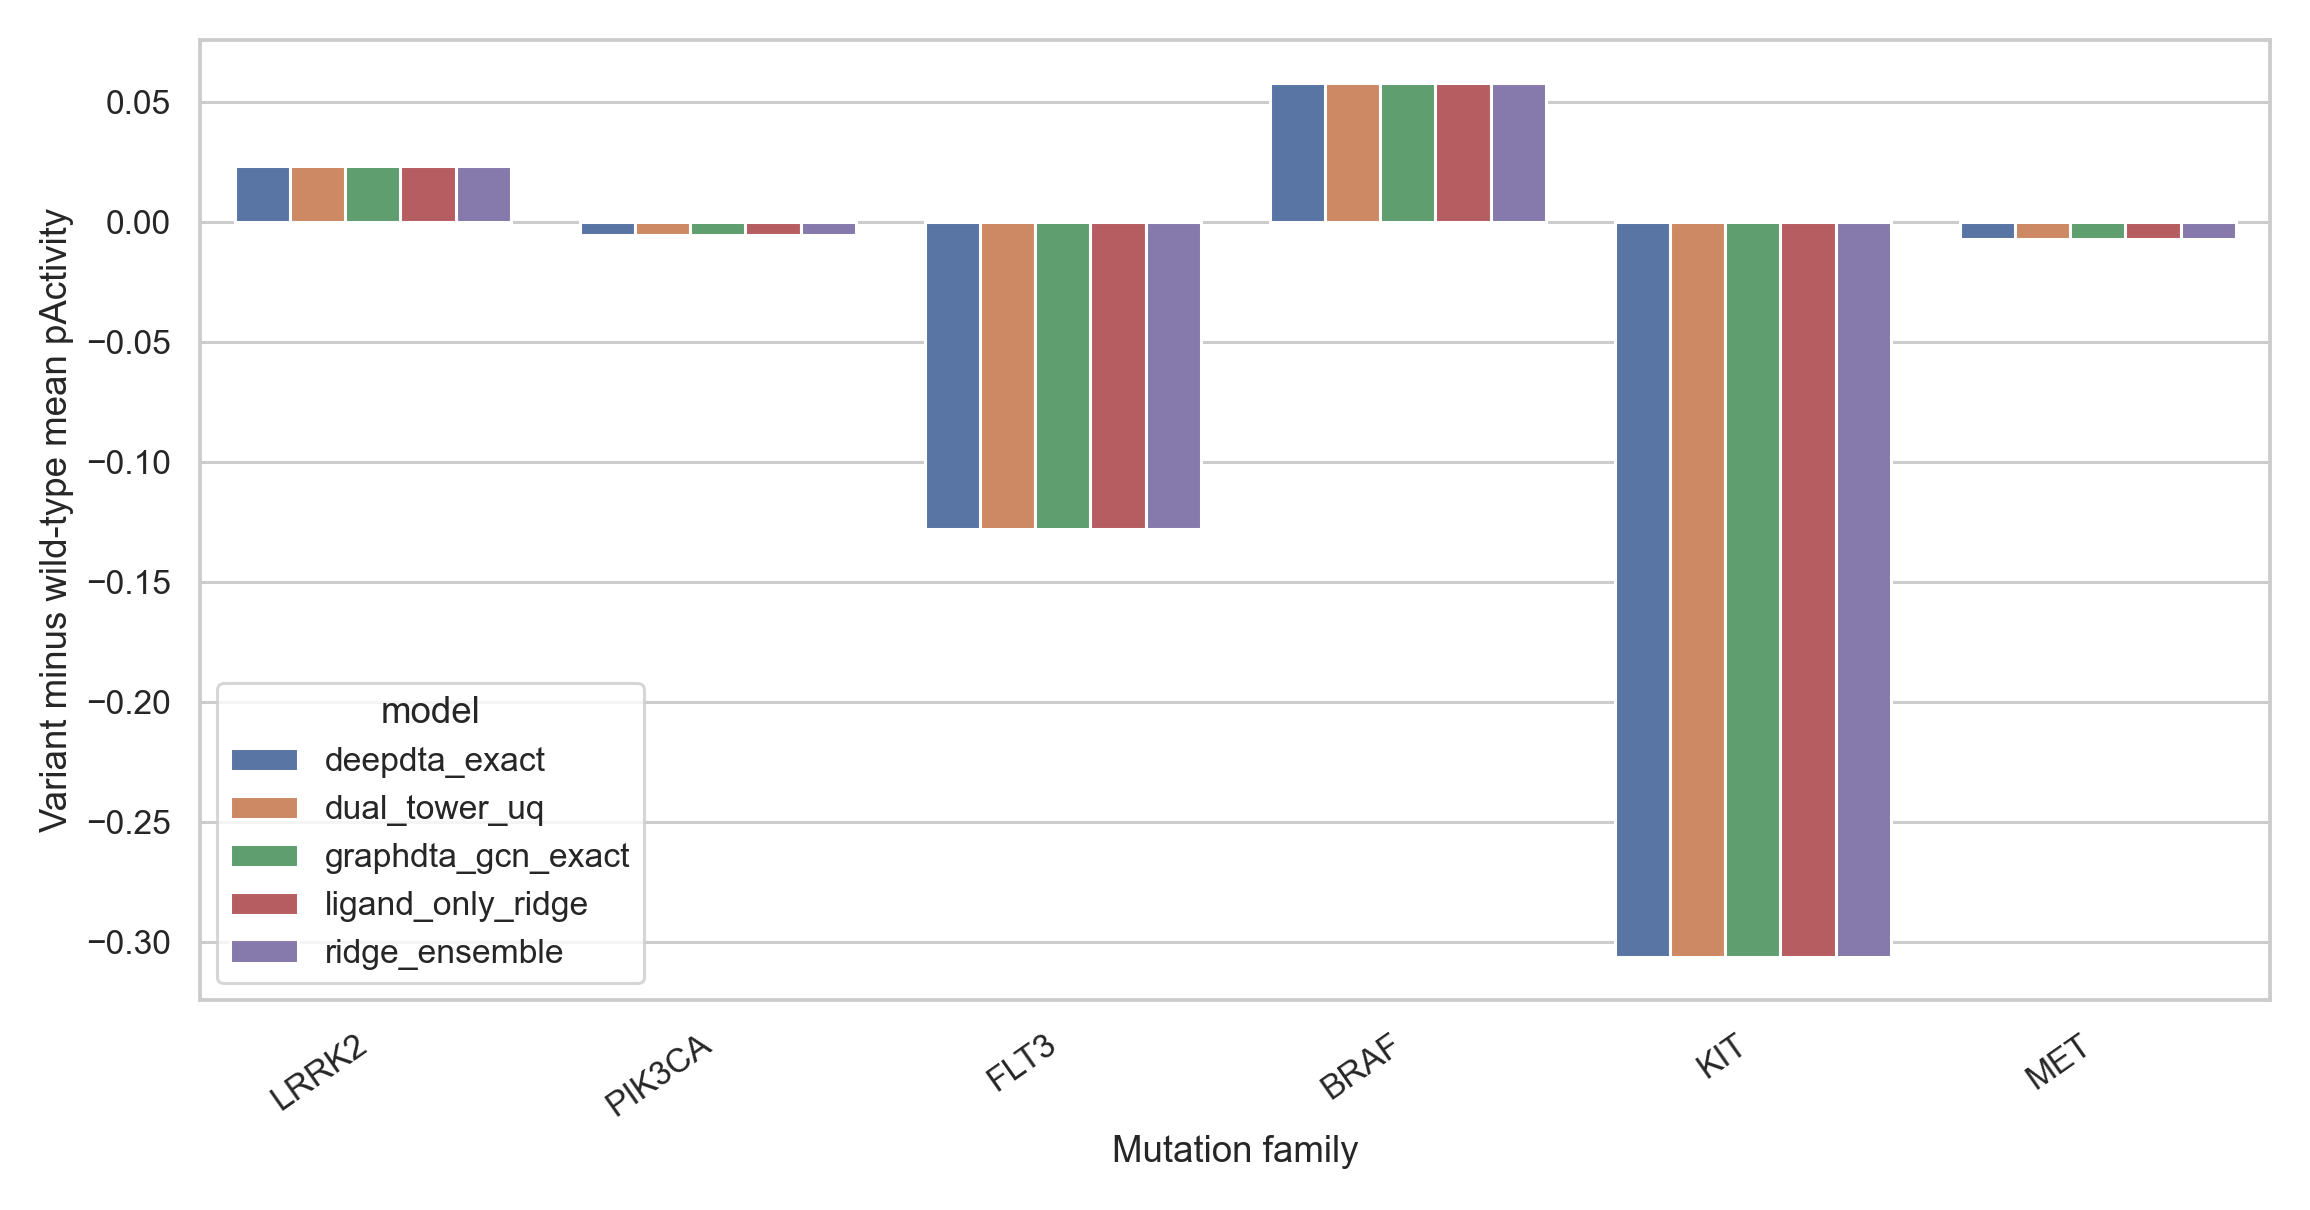
\includegraphics[width=0.85\linewidth]{../figures/mutation_family_delta.png}
\caption{Variant-versus-wild-type activity deltas across major mutation
families.}
\label{fig:mutation}
\end{figure}

\subsection{External Validation}

External validation on the BindingDB-derived kinase panel is harder than
in-domain Davis testing, but it is also more realistic. The current generated
external summary shows:

\begin{itemize}[leftmargin=1.5em]
  \item \texttt{dual\_tower\_uq}: RMSE 1.484, mean per-target Spearman 0.342
  \item \texttt{ridge\_ensemble}: RMSE 1.602, mean per-target Spearman 0.155
  \item \texttt{ligand\_only\_ridge}: RMSE 1.641, mean per-target Spearman 0.166
\end{itemize}

These numbers are worse than the in-domain Davis results, which is expected.
They should be interpreted as a more honest estimate of transfer difficulty.

\begin{figure}[H]
\centering
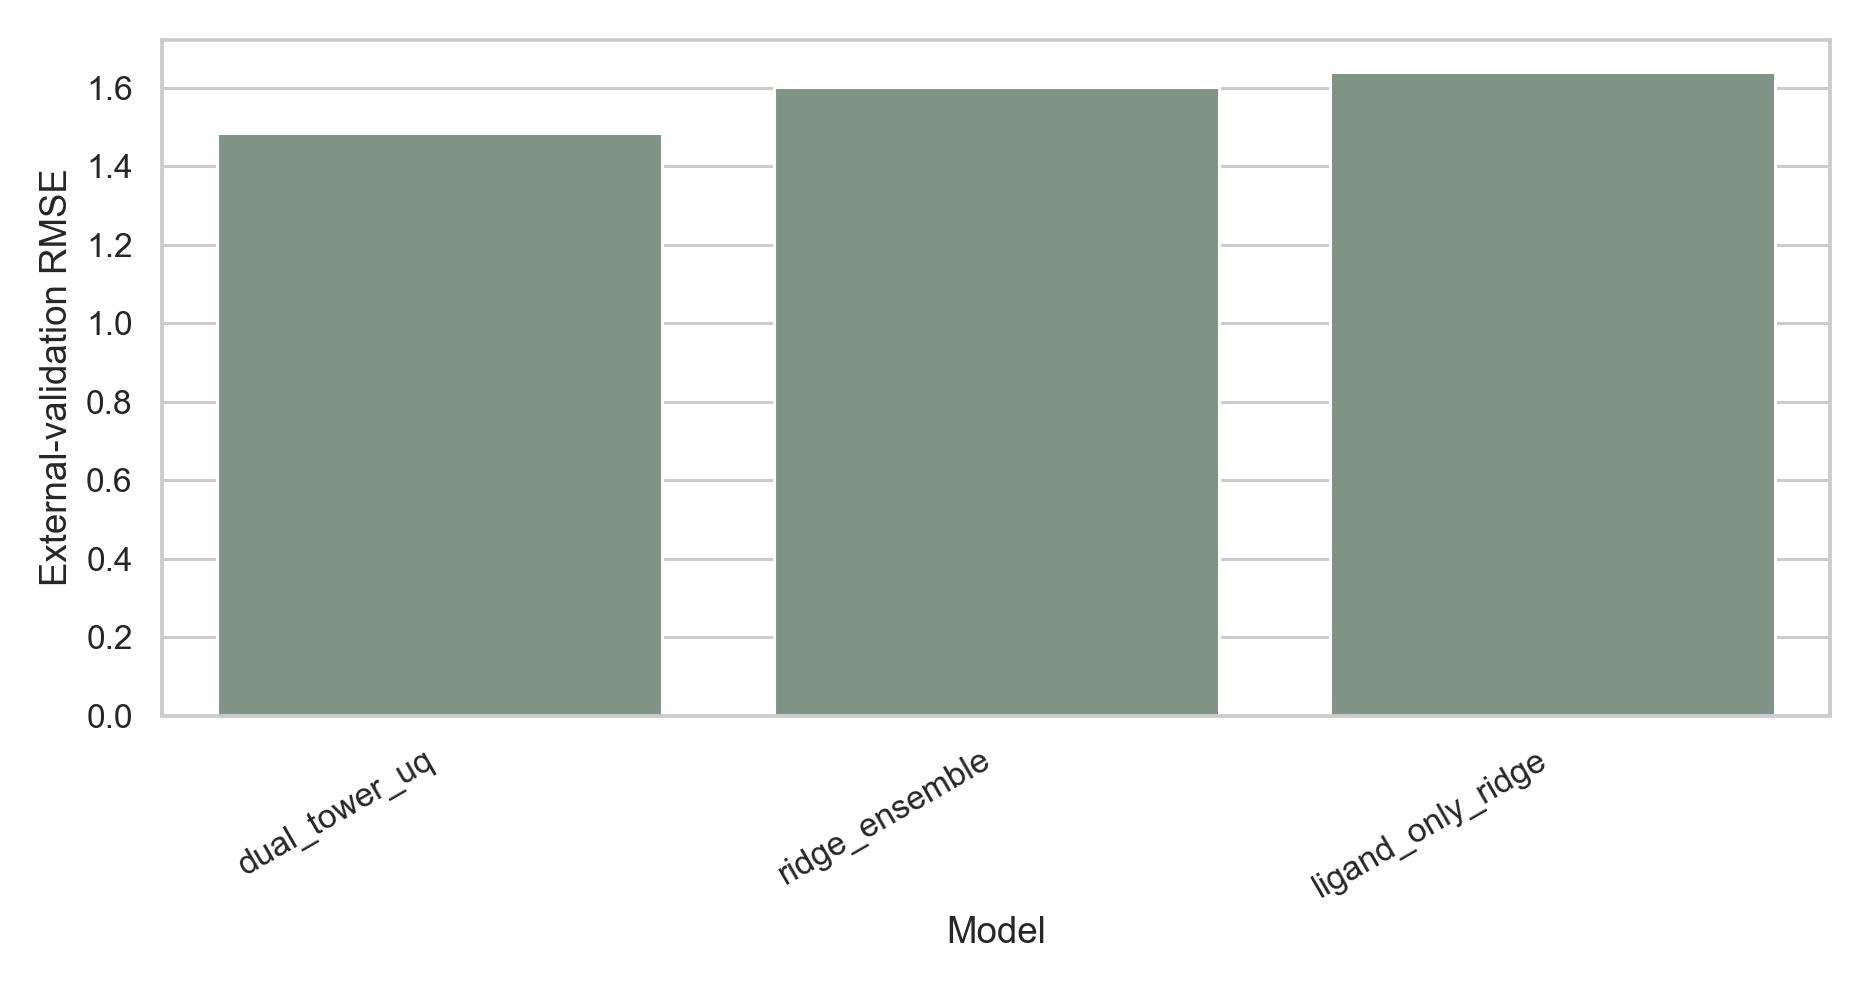
\includegraphics[width=0.75\linewidth]{../figures/external_validation_rmse.png}
\caption{External validation RMSE on the BindingDB-derived kinase panel.}
\label{fig:external}
\end{figure}

\subsection{Visual Summary of Main Split Results}

\begin{figure}[H]
\centering
\begin{subfigure}{0.88\linewidth}
  \centering
  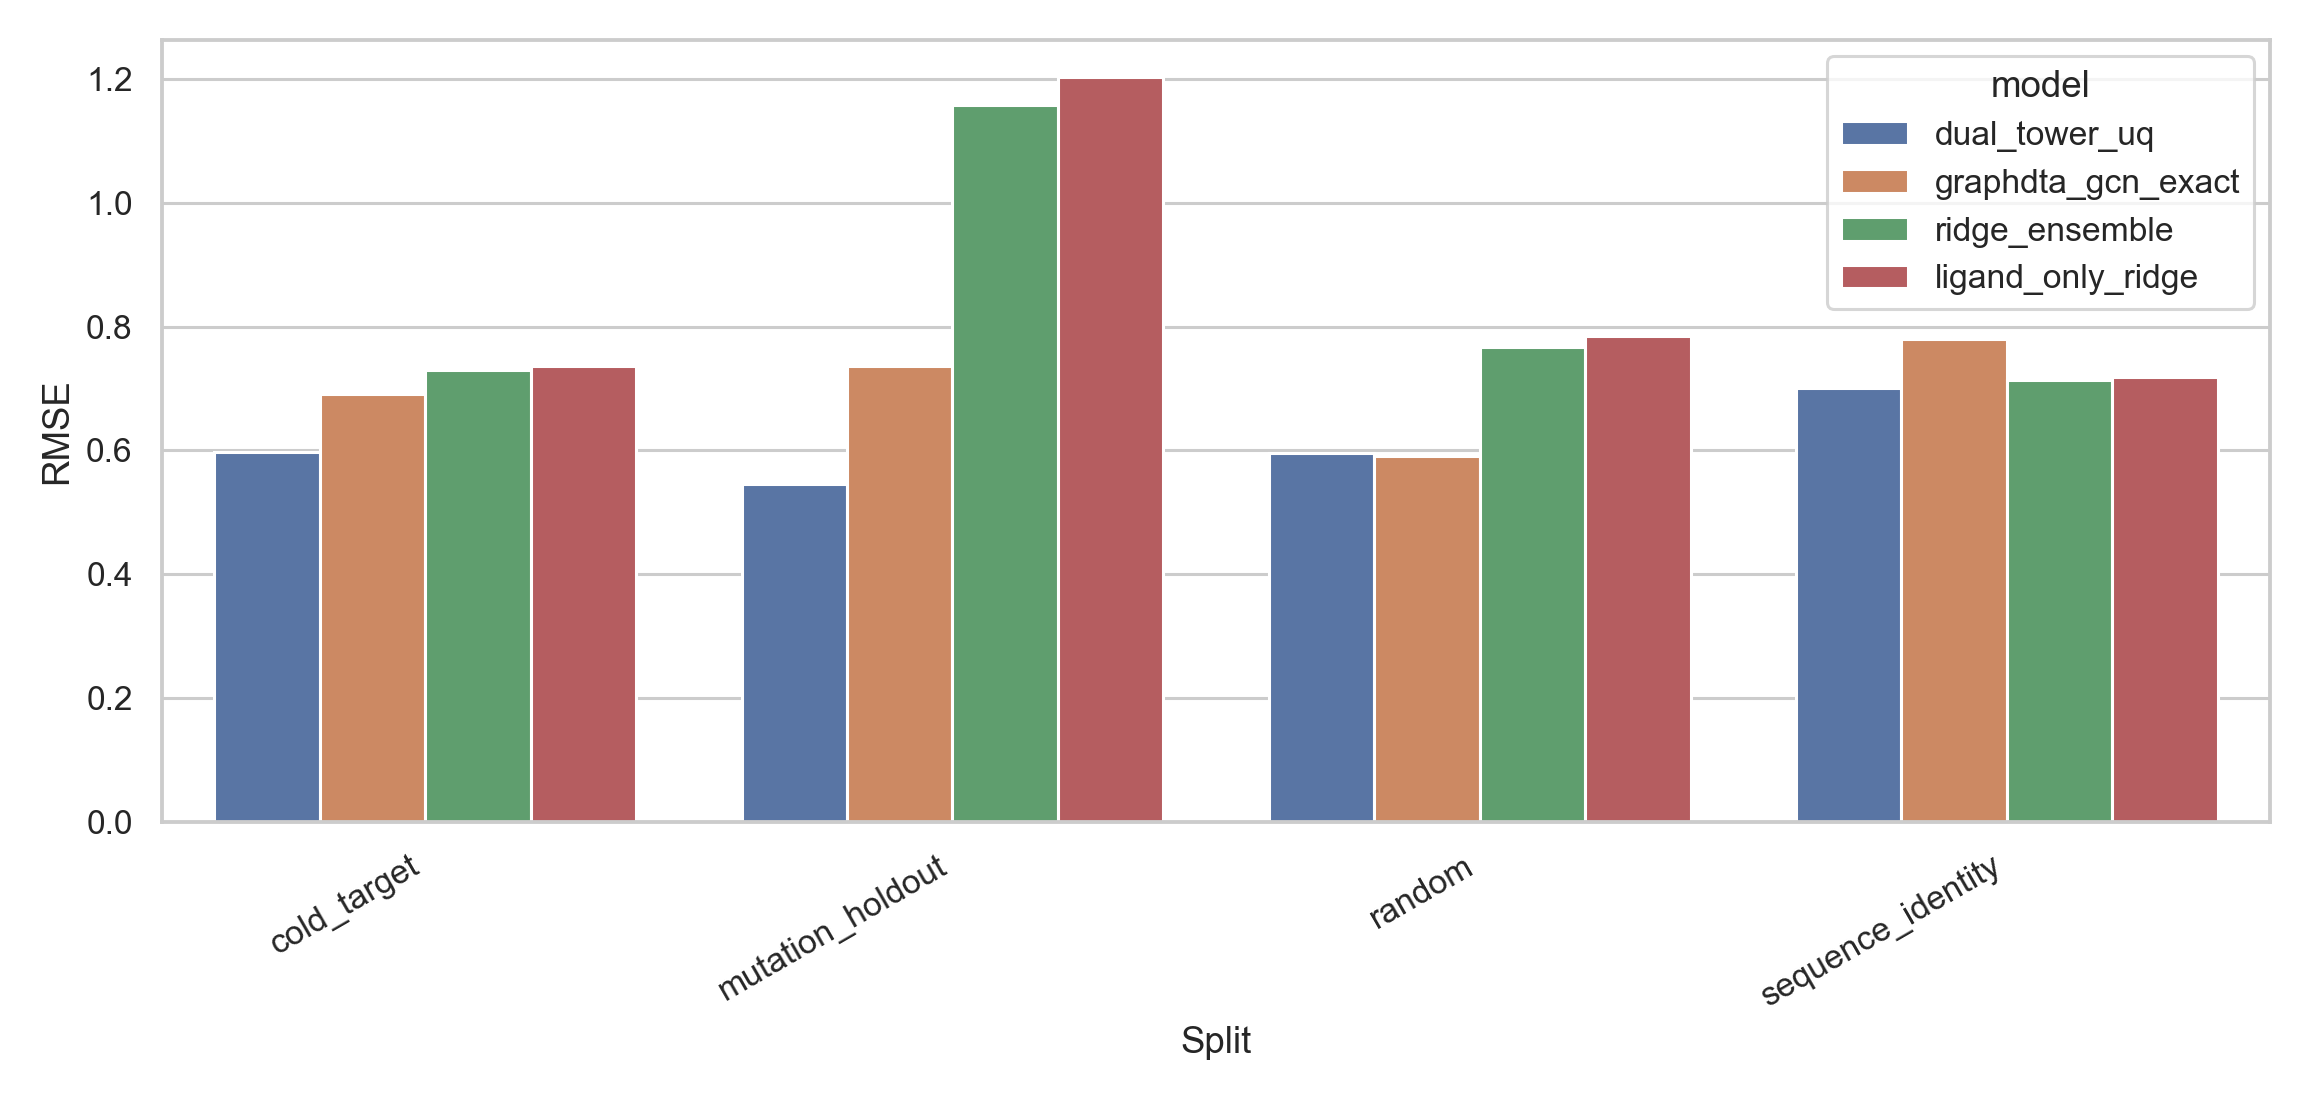
\includegraphics[width=\linewidth]{../figures/split_rmse_comparison.png}
  \caption{RMSE comparison.}
\end{subfigure}

\vspace{0.5em}

\begin{subfigure}{0.88\linewidth}
  \centering
  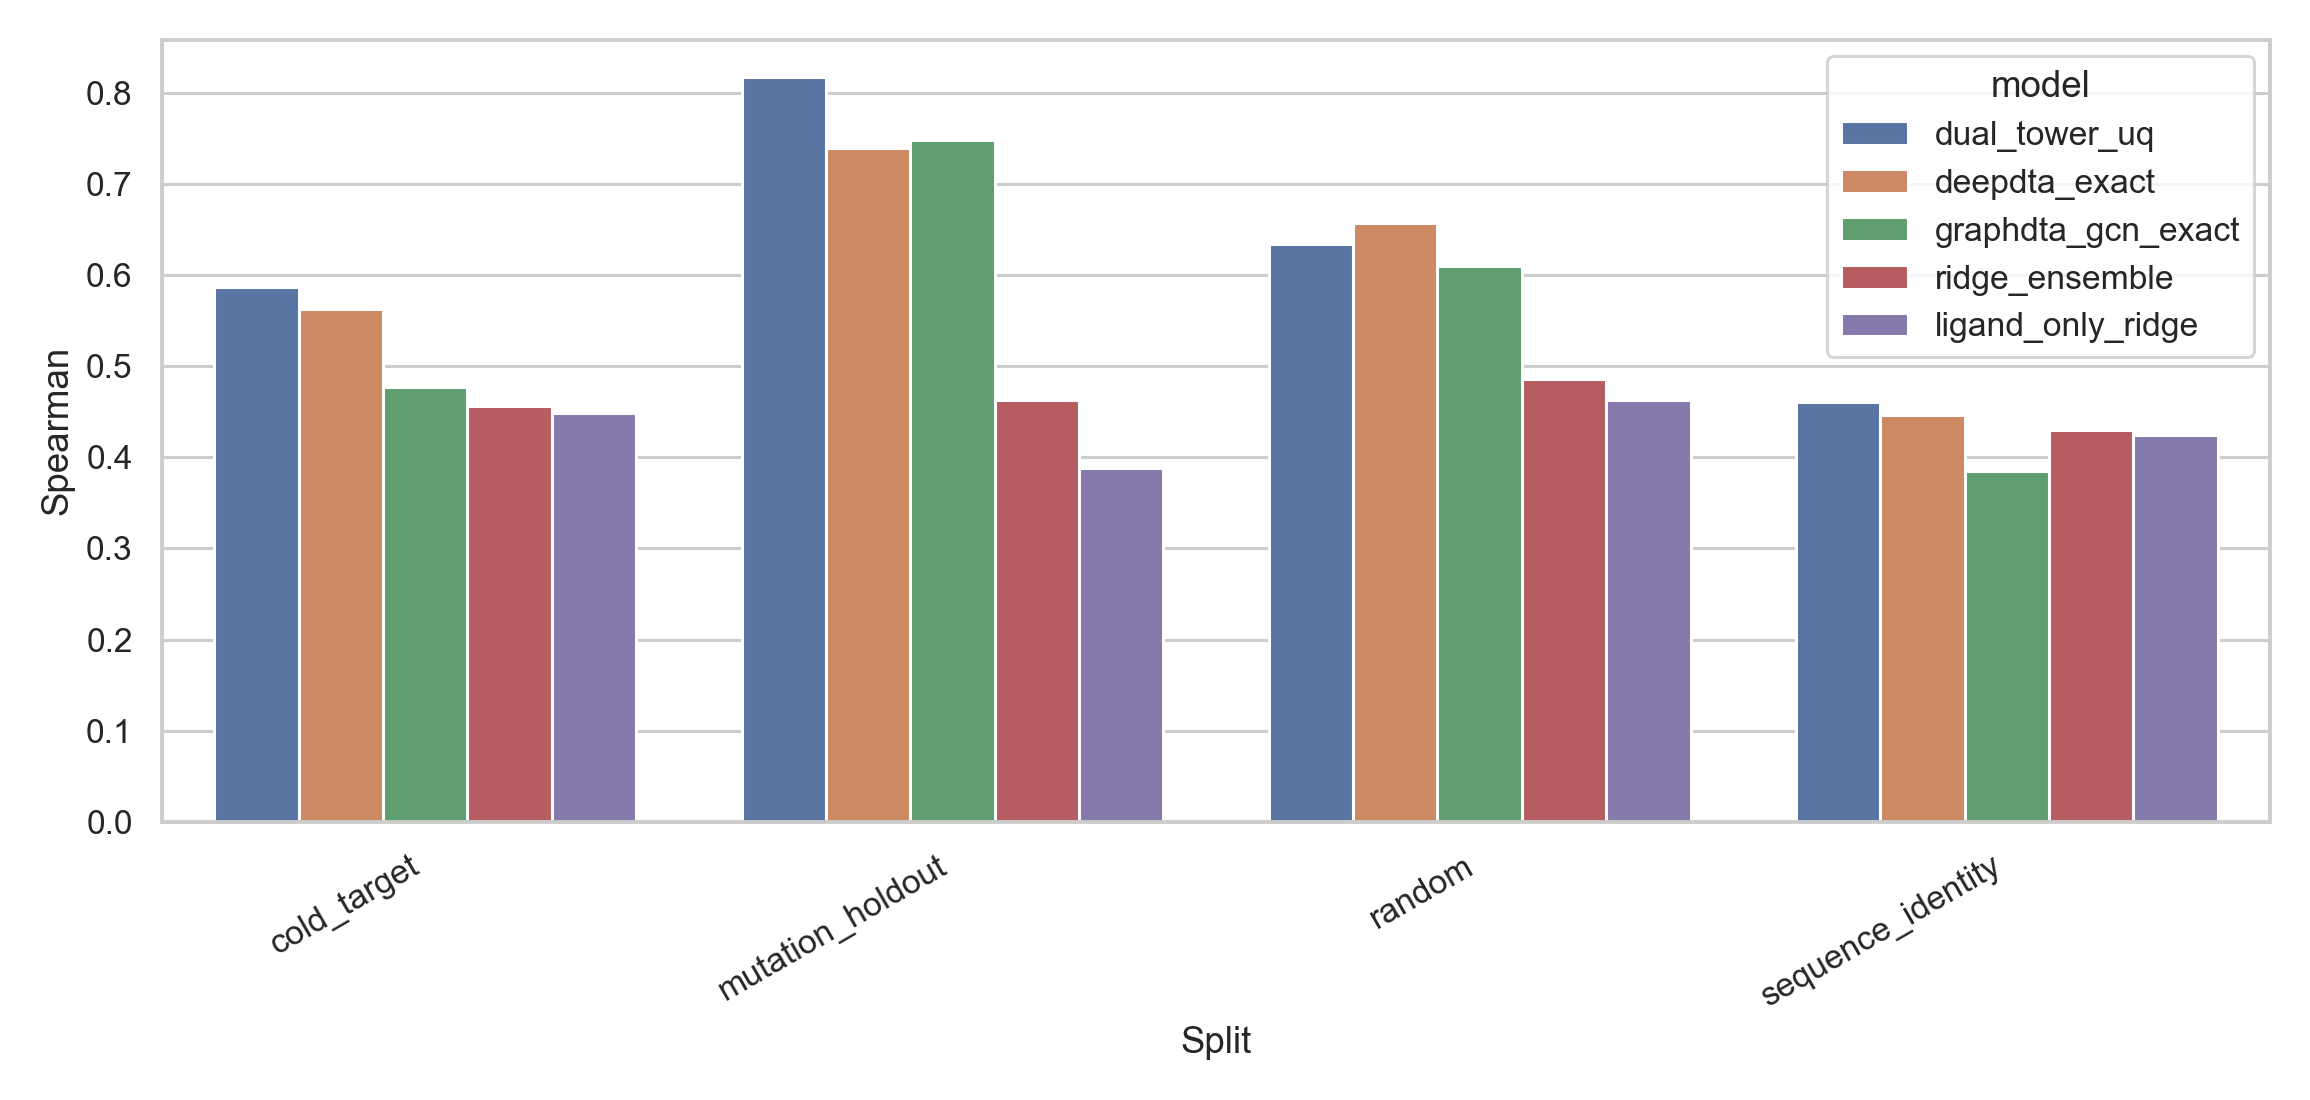
\includegraphics[width=\linewidth]{../figures/split_spearman_comparison.png}
  \caption{Spearman comparison.}
\end{subfigure}
\caption{Primary split-level benchmark summaries.}
\label{fig:main-benchmark}
\end{figure}

\section{Discussion}

The current evidence supports a stronger benchmark claim than a strongest-model
claim. The repository does not support the simplistic statement that its
primary model dominates every comparison. Instead, it supports a more credible
conclusion: the benchmark is realistic enough to produce meaningful trade-offs,
and the repository's \texttt{dual\_tower\_uq} model remains especially strong
on several of the harder settings, even in the presence of competitive
literature baselines.

This is arguably a better outcome for a benchmark paper. If every result
favored the repository model by a large margin under every split, reviewers
would reasonably ask whether the benchmark was tailored to the proposed method.
Instead, the current outcome suggests that split design matters, model ranking
depends on the evaluation regime, and realistic kinase prioritization should
not be reduced to one easy holdout.

\section{Repository Map}

The most important scientist-facing files are:

\begin{itemize}[leftmargin=1.5em]
  \item \texttt{scripts/run\_benchmark\_suite.py}: main benchmark runner
  \item \texttt{scripts/run\_external\_validation.py}: external validation
  runner
  \item \texttt{scripts/generate\_benchmark\_splits.py}: split generation
  \item \texttt{scripts/generate\_paper\_assets.py}: generated tables and
  figures
  \item \texttt{src/kinase\_ligand\_ranking/neural\_modeling.py}: repository
  model implementation
  \item \texttt{src/kinase\_ligand\_ranking/literature\_models.py}: DeepDTA and
  GraphDTA reproductions
\end{itemize}

\section{Limitations}

The current manuscript still has limitations. External validation artifacts are
currently strongest for the repository baselines; extending the same external
comparison to all literature baselines would further strengthen the story.
Similarly, repeated-seed results and confidence intervals would improve the
statistical presentation. These are strengthening steps rather than core
benchmark blockers.

\section{Conclusion}

KinBench-UQ is now more than a baseline repository. It provides a reproducible
evaluation stack for kinase candidate prioritization, with exact
sequence-identity-aware splitting, mutation-family analysis, external
validation, literature-style reproductions, and generated manuscript evidence.
The current results show that the benchmark meaningfully differentiates models:
\texttt{deepdta\_exact} is strongest on easier settings, while
\texttt{dual\_tower\_uq} is particularly strong on several harder and more
scientist-relevant evaluation regimes.

\end{document}
